% Manuscrito v4. Compilar con: xelatex -> biber -> xelatex -> xelatex
\documentclass[man,12pt,floatsintext,donotrepeattitle]{apa7}
\usepackage[spanish,es-noquoting,es-tabla,es-nolists]{babel}
\usepackage{fontspec}
\setmainfont{TeX Gyre Termes}
\usepackage{csquotes}
\usepackage[backend=biber,style=apa]{biblatex}
\DeclareLanguageMapping{spanish}{spanish-apa}
\usepackage{graphicx}
\usepackage{booktabs}
\usepackage{longtable}
\usepackage{array}
\usepackage{float}
\usepackage{caption}
\usepackage{hyperref}
\usepackage{amsmath}
\usepackage{amssymb}
\usepackage{xpatch}
% APA en español: "y" en lugar de "&" entre los dos últimos autores
\DeclareDelimFormat[bib,biblist]{finalnamedelim}{\ifthenelse{\value{listcount}>\maxprtauth}{}{\ifthenelse{\value{liststop}>2}{\finalandcomma\addspace\bibstring{and}\space}{\addspace\bibstring{and}\space}}}
\DeclareDelimFormat[parencite]{finalnamedelim}{\ifnum\value{liststop}>2 \finalandcomma\fi\addspace\bibstring{and}\space}
% Capítulos en libro editado: (Vol. x, pp. y-z), en ese orden
\xpatchbibmacro{addinfo1}{\ifentrytype{inbook}{\printfield{pages}}{}}{}{}{\PatchFailed}
\xpatchbibmacro{addinfo1}{\ifthenelse{\ifentrytype{book}\OR\ifentrytype{inbook}}{\printfield{volume}}{}}{\ifthenelse{\ifentrytype{book}\OR\ifentrytype{inbook}}{\printfield{volume}}{}\setunit*{\addcomma\addspace}\ifentrytype{inbook}{\printfield{pages}}{}}{}{\PatchFailed}
\addbibresource{referencias.bib}
\hypersetup{hidelinks}
\urlstyle{same}
\def\acksname{Nota del autor}
% Flujo continuo: sin estirar el espacio vertical, sin líneas viudas ni huérfanas
\raggedbottom
\widowpenalty=10000
\clubpenalty=10000
\captionsetup{skip=6pt}

\title{Sistemas Conversacionales Anclados en Recuperación para el Acceso a Información Normativa y Procedimental en Instituciones de Educación Superior: Una Revisión Sistemática}
\shorttitle{RAG para información normativa universitaria}
\author{Edgar David Mariano Ruiz, Arnulfo Catalán Villegas y Mercedes Hernández De La Cruz}
\affiliation{Facultad de Ingeniería, Universidad Autónoma de Guerrero\\Maestría en Ingeniería para la Innovación y el Desarrollo Tecnológico\\Octubre de 2026}
\authornote{Edgar David Mariano Ruiz, Facultad de Ingeniería, Universidad Autónoma de Guerrero. Arnulfo Catalán Villegas, Facultad de Ingeniería, Universidad Autónoma de Guerrero. Mercedes Hernández De La Cruz, Facultad de Ingeniería, Universidad Autónoma de Guerrero.

Correspondencia: Edgar David Mariano Ruiz, Facultad de Ingeniería, Universidad Autónoma de Guerrero, Chilpancingo de los Bravo, Guerrero, México. Correo: 25600451@uagro.mx. ORCID: \url{https://orcid.org/0009-0005-6171-1206}.

Los autores declaran no tener conflictos de intereses.

El protocolo congelado, las cadenas de búsqueda, la matriz de extracción y el formulario de calidad están disponibles en \url{https://github.com/DavidMariano300/rsl-rag-normativa-universitaria}.}

\begin{document}
\maketitle
\section*{Resumen}
\noindent Las universidades acumulan un acervo normativo extenso y difícil de consultar. Esta revisión sistemática valoró la evidencia empírica sobre sistemas conversacionales anclados en recuperación aplicados a ese acervo, con atención a la fidelidad de las respuestas y al tiempo de consulta. Se siguieron PRISMA 2020 y las guías de Kitchenham y Charters. De 2\,179 registros recuperados en cuatro fuentes, la indización editorial de cada candidato se verificó por el prefijo de su identificador digital de objeto; 90 estudios pasaron a cribado, 30 a texto completo y 28 a extracción, y 24 superaron el umbral de calidad de 4.0 sobre 7.0. La estrategia de segmentación del documento se declara en 20 de los 24 estudios y solo dos la prueban experimentalmente; en ellos, los fragmentos de 512 unidades léxicas superan a los de 4\,000 y resumir el fragmento degrada la recuperación y la respuesta. Las métricas de clasificación dominan la evaluación (12 de 24) y la fidelidad, cuando se mide aparte, es la puntuación más baja. Ocho estudios reportan latencia y ninguno la compara contra la consulta tradicional. La respuesta cita su fuente en 9 estudios y solo 4 publican datos o código. Ningún estudio trabaja con un corpus en español ni proviene de América Latina. El anclaje documental reduce la invención de datos; falta demostrar que reduce el tiempo de acceso a la norma. La segmentación del documento normativo en español y la medición del tiempo con un diseño de dos brazos son las líneas de mayor retorno.
\par\indent\textit{Palabras clave:} generación anclada en recuperación, información normativa universitaria, evaluación de fidelidad, segmentación semántica, trazabilidad documental, revisión sistemática

\section*{Abstract}
\noindent Universities hold an extensive body of institutional regulation that governs the daily decisions of students, applicants and staff, and that is hard to consult. This systematic review appraised the empirical evidence on retrieval-augmented conversational systems applied to that body of regulation, focusing on how answer faithfulness was evaluated and on consultation time. PRISMA 2020 and the Kitchenham and Charters guidelines were followed. From 2,179 records retrieved from four sources, the publisher indexing of every candidate was verified through its digital object identifier prefix; 90 studies entered screening, 30 were assessed in full text, 28 were extracted, and 24 passed a quality threshold of 4.0 out of 7.0. Document segmentation strategy was reported in 20 of the 24 studies and only two tested it experimentally; in those, 512-token chunks outperformed 4,000-token chunks and summarizing the chunk degraded both retrieval and answers. Classification metrics dominated evaluation (12 of 24), and faithfulness, when measured separately, was the lowest score reported. Eight studies reported latency and none compared it against traditional consultation. Answers cited their source in 9 studies and only 4 released data or code. No study used a Spanish-language corpus or came from Latin America. Document grounding reduces fabricated content; whether it reduces the time needed to reach a regulation remains to be shown. Segmentation of Spanish-language regulatory documents and the measurement of consultation time with a two-arm design are the lines with the greatest return.
\par\indent\textit{Keywords:} retrieval-augmented generation, university regulation, faithfulness evaluation, semantic chunking, document traceability, systematic review

\section*{\normalfont\textbf{Sistemas Conversacionales Anclados en Recuperación para el Acceso a Información Normativa y Procedimental en Instituciones de Educación Superior: Una Revisión Sistemática}}
\section{Introducción}
Una universidad pública mexicana de tamaño medio administra decenas de documentos normativos vigentes, desde la ley orgánica y el estatuto hasta los reglamentos de titulación, los lineamientos de becas y las convocatorias anuales, y ese acervo cambia por partes y a destiempo. Quien necesita saber cuántas veces puede recursar una asignatura no enfrenta falta de información. Enfrenta un problema de localización: la respuesta es pública, pero vive en un artículo concreto de un documento concreto, y la ventanilla que podría orientarlo tiene horario y depende del personal en turno.

La generación anclada en recuperación, conocida por sus siglas en inglés como RAG, ofrece una vía técnica para ese problema. En lugar de confiar en lo que un modelo de lenguaje memorizó durante su entrenamiento, el sistema recupera primero los fragmentos pertinentes de un corpus propio y después pide al modelo que redacte la respuesta con ese material. Para el dominio normativo esto tiene dos atractivos claros: la respuesta puede citar su fuente, y el corpus se actualiza sin reentrenar nada.

Entre 2024 y 2026 aparecieron numerosas implementaciones de esta idea en universidades. La evidencia de que el anclaje reduce la invención de datos es consistente, así que esta revisión se pregunta otra cosa: si esa literatura contesta lo que un proyecto institucional necesita saber antes de comprometer recursos. Interesa cómo conviene segmentar un corpus normativo, con qué instrumento se comprueba que la respuesta es fiel al documento y no una paráfrasis plausible, y si alguien ha medido que el sistema reduce el tiempo de consulta frente a la ventanilla.

\subsection{Preguntas de Investigación}
La formulación sigue la estructura PICOC. La población son las instituciones de educación superior y sus usuarios. La intervención son los sistemas conversacionales cuya generación está anclada en un corpus institucional recuperado, comparados con los mecanismos tradicionales de consulta o con configuraciones alternativas del propio sistema. Los resultados de interés son la fidelidad o precisión factual, el tiempo de respuesta, la usabilidad y la satisfacción, en el contexto de la información normativa, administrativa y procedimental de la institución.

\textbf{PI1.} ¿Qué arquitecturas de recuperación y generación se han implementado para el acceso a información normativa y administrativa en educación superior, y cómo se preparan los corpus documentales que las alimentan?

\textbf{PI2.} ¿Con qué métricas, instrumentos y procedimientos se evalúa la fidelidad de las respuestas, y qué valores se reportan?

\textbf{PI3.} ¿Qué evidencia empírica existe sobre la reducción del tiempo de acceso a la información frente a los mecanismos tradicionales de consulta?

\textbf{PI4.} ¿Qué prácticas de reporte y qué vacíos metodológicos presentan los estudios en cuanto a trazabilidad de la respuesta, disponibilidad de datos y reproducibilidad?

Esta revisión constituye el marco de evidencia de la tesis de maestría del primer autor, cuyo objetivo es diseñar e implementar un sistema conversacional anclado en recuperación para el acceso a información normativa de la Universidad Autónoma de Guerrero.

\section{Método}
El protocolo se congeló antes de ejecutar la primera búsqueda y cada desviación posterior quedó asentada, con fecha y justificación, en su bitácora. El reporte sigue la declaración PRISMA 2020 \parencite{page2021}. El diseño se apoya en las guías de \textcite{kitchenham2007} para revisiones sistemáticas en ingeniería de software y, para la búsqueda por citas, en \textcite{wohlin2014}.

\subsection{Fuentes y Verificación de Indización}
Las cinco bases previstas como primarias (Scopus, Web of Science, IEEE Xplore, ACM Digital Library y SpringerLink) se sometieron a una prueba de consulta automatizada el 4 de septiembre de 2026. Ninguna la admitió sin credenciales institucionales. Scopus, Web of Science y SpringerLink devolvieron error de autorización; IEEE y ACM, error de acceso prohibido. La limitación quedó documentada en el protocolo y llevó a un procedimiento de dos pasos.

La recuperación se ejecutó sobre fuentes de consulta abierta. OpenAlex y Crossref funcionaron como agregadores de metadatos, y ERIC y DBLP como bases especializadas y curadas. Después, cada registro pasó por una verificación editorial basada en el prefijo de su identificador digital de objeto, que identifica sin ambigüedad a la agencia que lo registró: 10.1109 corresponde al Institute of Electrical and Electronics Engineers, 10.1145 a la Association for Computing Machinery, 10.1007 a Springer Nature, 10.1016 a Elsevier y 10.3390 a MDPI. Se descartó todo registro cuyo prefijo no correspondiera a una plataforma con indización reconocida.

El prefijo prueba quién publicó el trabajo y en qué plataforma editorial está alojado. No prueba que esté indizado en Scopus o en Web of Science, que son servicios distintos. Por eso esta revisión afirma que cada estudio incluido está publicado por IEEE, ACM, Springer, Elsevier o MDPI, y deja la verificación directa en las bases de indización como tarea pendiente.

\subsection{Cadenas de Búsqueda}
La cadena base combina tres bloques por conjunción, cada uno con sus sinónimos unidos por disyunción, y se aplicó sobre título, resumen y palabras clave. El bloque de tecnología cubre \texttt{\textquotedbl{}retrieval augmented generation\textquotedbl{} OR \textquotedbl{}retrieval-augmented generation\textquotedbl{} OR RAG OR \textquotedbl{}grounded generation\textquotedbl{} OR \textquotedbl{}retrieval grounded\textquotedbl{}}. El de sistema conversacional cubre \texttt{chatbot OR \textquotedbl{}conversational agent\textquotedbl{} OR \textquotedbl{}conversational assistant\textquotedbl{} OR \textquotedbl{}virtual assistant\textquotedbl{} OR \textquotedbl{}question answering\textquotedbl{} OR \textquotedbl{}dialogue system\textquotedbl{}}. El de contexto institucional combina \texttt{university OR \textquotedbl{}higher education\textquotedbl{} OR campus OR \textquotedbl{}academic institution\textquotedbl{}} con \texttt{regulation* OR normative OR policy OR bylaw* OR statute OR administrative OR enrollment OR admission OR registrar OR \textquotedbl{}student services\textquotedbl{} OR procedure*}.

Para no perder estudios con vocabulario distinto, la búsqueda se amplió a seis variantes de la cadena, relajando un bloque a la vez. Sobre los registros de Crossref la cadena se aplicó después de la descarga, de forma determinista, sobre título y resumen. Se complementó con rastreo de citas hacia atrás y hacia adelante sobre los estudios incluidos \parencite{wohlin2014}.

\subsection{Criterios de Elegibilidad}
Un estudio se incluyó si cumplía los ocho criterios de inclusión y ninguno de los de exclusión (Tabla 1).

{\def\baselinestretch{1}\small\selectfont
\begin{longtable}{@{}>{\raggedright\arraybackslash}p{0.085\linewidth}>{\raggedright\arraybackslash}p{0.273\linewidth}>{\raggedright\arraybackslash}p{0.583\linewidth}@{}}
\caption{Criterios de Elegibilidad}\label{tab:1}\\
\toprule
Código & Criterio & Definición \\
\midrule
\endfirsthead
\multicolumn{3}{@{}l}{\textit{Tabla 1 (continuación)}}\\
\toprule
Código & Criterio & Definición \\
\midrule
\endhead
I1 & Estudio primario con RAG & Desarrolla, implementa o evalúa un sistema cuya generación está anclada en documentos recuperados \\
I2 & Educación superior & El sistema se aplica en una institución de educación superior \\
I3 & Información institucional & La información objetivo es normativa, administrativa o procedimental de la institución \\
I4 & Evaluación empírica & Reporta al menos una métrica cuantitativa o un instrumento sistemático de valoración \\
I5 & Periodo & Publicado entre 2022 y 2026 \\
I6 & Revisión por pares & Publicado en revista o en congreso con comité científico \\
I7 & Idioma y acceso & Texto completo accesible en inglés o en español \\
I8 & Indización editorial & Alojado en una plataforma editorial con indización reconocida \\
E1 & Contenido instruccional & El objeto es tutoría, contenido de curso o apoyo al aprendizaje \\
E2 & Sin corpus propio & El sistema no recupera sobre un corpus institucional \\
E3 & Estudio secundario & Revisión, mapeo sistemático o metaanálisis \\
E4 & Literatura gris & Preimpresión, tesis, reporte técnico o documentación de producto \\
E5 & Otro dominio & Dominio clínico, industrial, jurisdiccional o corporativo \\
E6 & Sin evaluación & No presenta evaluación empírica o solo describe una arquitectura \\
E7 & Duplicado & Versión duplicada o preliminar de un trabajo ya incluido \\
E8 & Editorial no indizada & Publicado por una editorial sin plataforma de indización reconocida \\
\bottomrule
\end{longtable}}
\vspace{-1.2em}
{\footnotesize\noindent\textit{Nota.} La indización editorial de los criterios I8 y E8 se comprobó por el prefijo del identificador digital de objeto.\par}
\vspace{1em}

\subsection{Evaluación de la Calidad}
Cada estudio incluido se puntuó con un instrumento de siete criterios adaptado de \textcite{kitchenham2007} y de \textcite{dyba2008}. Un criterio vale 1 punto si se cumple, 0.5 si se cumple de forma parcial y 0 si no se cumple. Los criterios valoran si el estudio declara con claridad sus objetivos (QA1), si describe el corpus de manera que su preparación sea replicable (QA2), si especifica la arquitectura con detalle suficiente para reproducirla (QA3), si reporta evaluación empírica con métricas definidas y procedimiento descrito (QA4), si incluye una línea base o configuración alternativa (QA5), si discute limitaciones y amenazas a la validez (QA6) y si pone a disposición datos, código o conjunto de evaluación (QA7).

La puntuación máxima es 7.0. El umbral de inclusión en la síntesis, fijado antes de puntuar, es 4.0, y los estudios por debajo se reportan aparte con su puntuación y su motivo.

\subsection{Extracción de Datos}
El formulario de extracción tiene once grupos de campos: identificación, contexto, corpus, segmentación, recuperación, generación, evaluación, resultados, comparación, trazabilidad y reproducibilidad, más las limitaciones declaradas y la puntuación de calidad. La extracción se realizó leyendo el texto completo de cada estudio. Como apoyo operativo se construyó una versión condensada que conservaba encabezados y líneas técnicas, pero los valores numéricos, los tamaños de conjunto y las secciones de limitaciones se verificaron siempre contra el texto íntegro. La matriz resultante tiene 28 estudios por 34 campos y no contiene celdas vacías.

\subsection{Número de Revisores}
El cribado, la extracción y la puntuación de calidad los realizó el primer autor. El protocolo original previó doble cribado independiente, pero la restricción de recursos del programa de maestría impidió cumplir esa previsión. Como compensación, la puntuación de cada criterio de cada estudio se publica en el repositorio del proyecto con la regla aplicada y la evidencia extraída, y los cuatro estudios excluidos por calidad se reportan con su puntuación y su motivo específico, de modo que la decisión pueda impugnarse. El director de tesis validó el conjunto seleccionado y el procedimiento de extracción. El coeficiente kappa no se calculó.

\section{Resultados}
\subsection{Selección de Estudios}
La búsqueda en bases recuperó 2\,179 registros: 1\,676 de OpenAlex con las seis variantes de la cadena, 450 de Crossref, 42 de ERIC y 11 de DBLP. Tras eliminar 760 duplicados quedaron 1\,419 registros únicos, de los cuales 1\,168 no contenían los bloques de la cadena en título y resumen. De los 251 restantes, 217 venían del flujo de OpenAlex y Crossref, y 161 de ellos estaban publicados por editoriales sin plataforma indizada. Quedaron 56 registros de ese flujo y 34 de ERIC y DBLP. El rastreo de citas examinó 692 registros y aportó 2 estudios nuevos. Tras eliminar 2 duplicados en la consolidación, 90 registros pasaron a cribado por título y resumen (Figura 1).

\begin{figure}[htbp]
\caption{Diagrama de Flujo PRISMA 2020 de la Revisión Sistemática}
\label{fig:prisma}
\centering
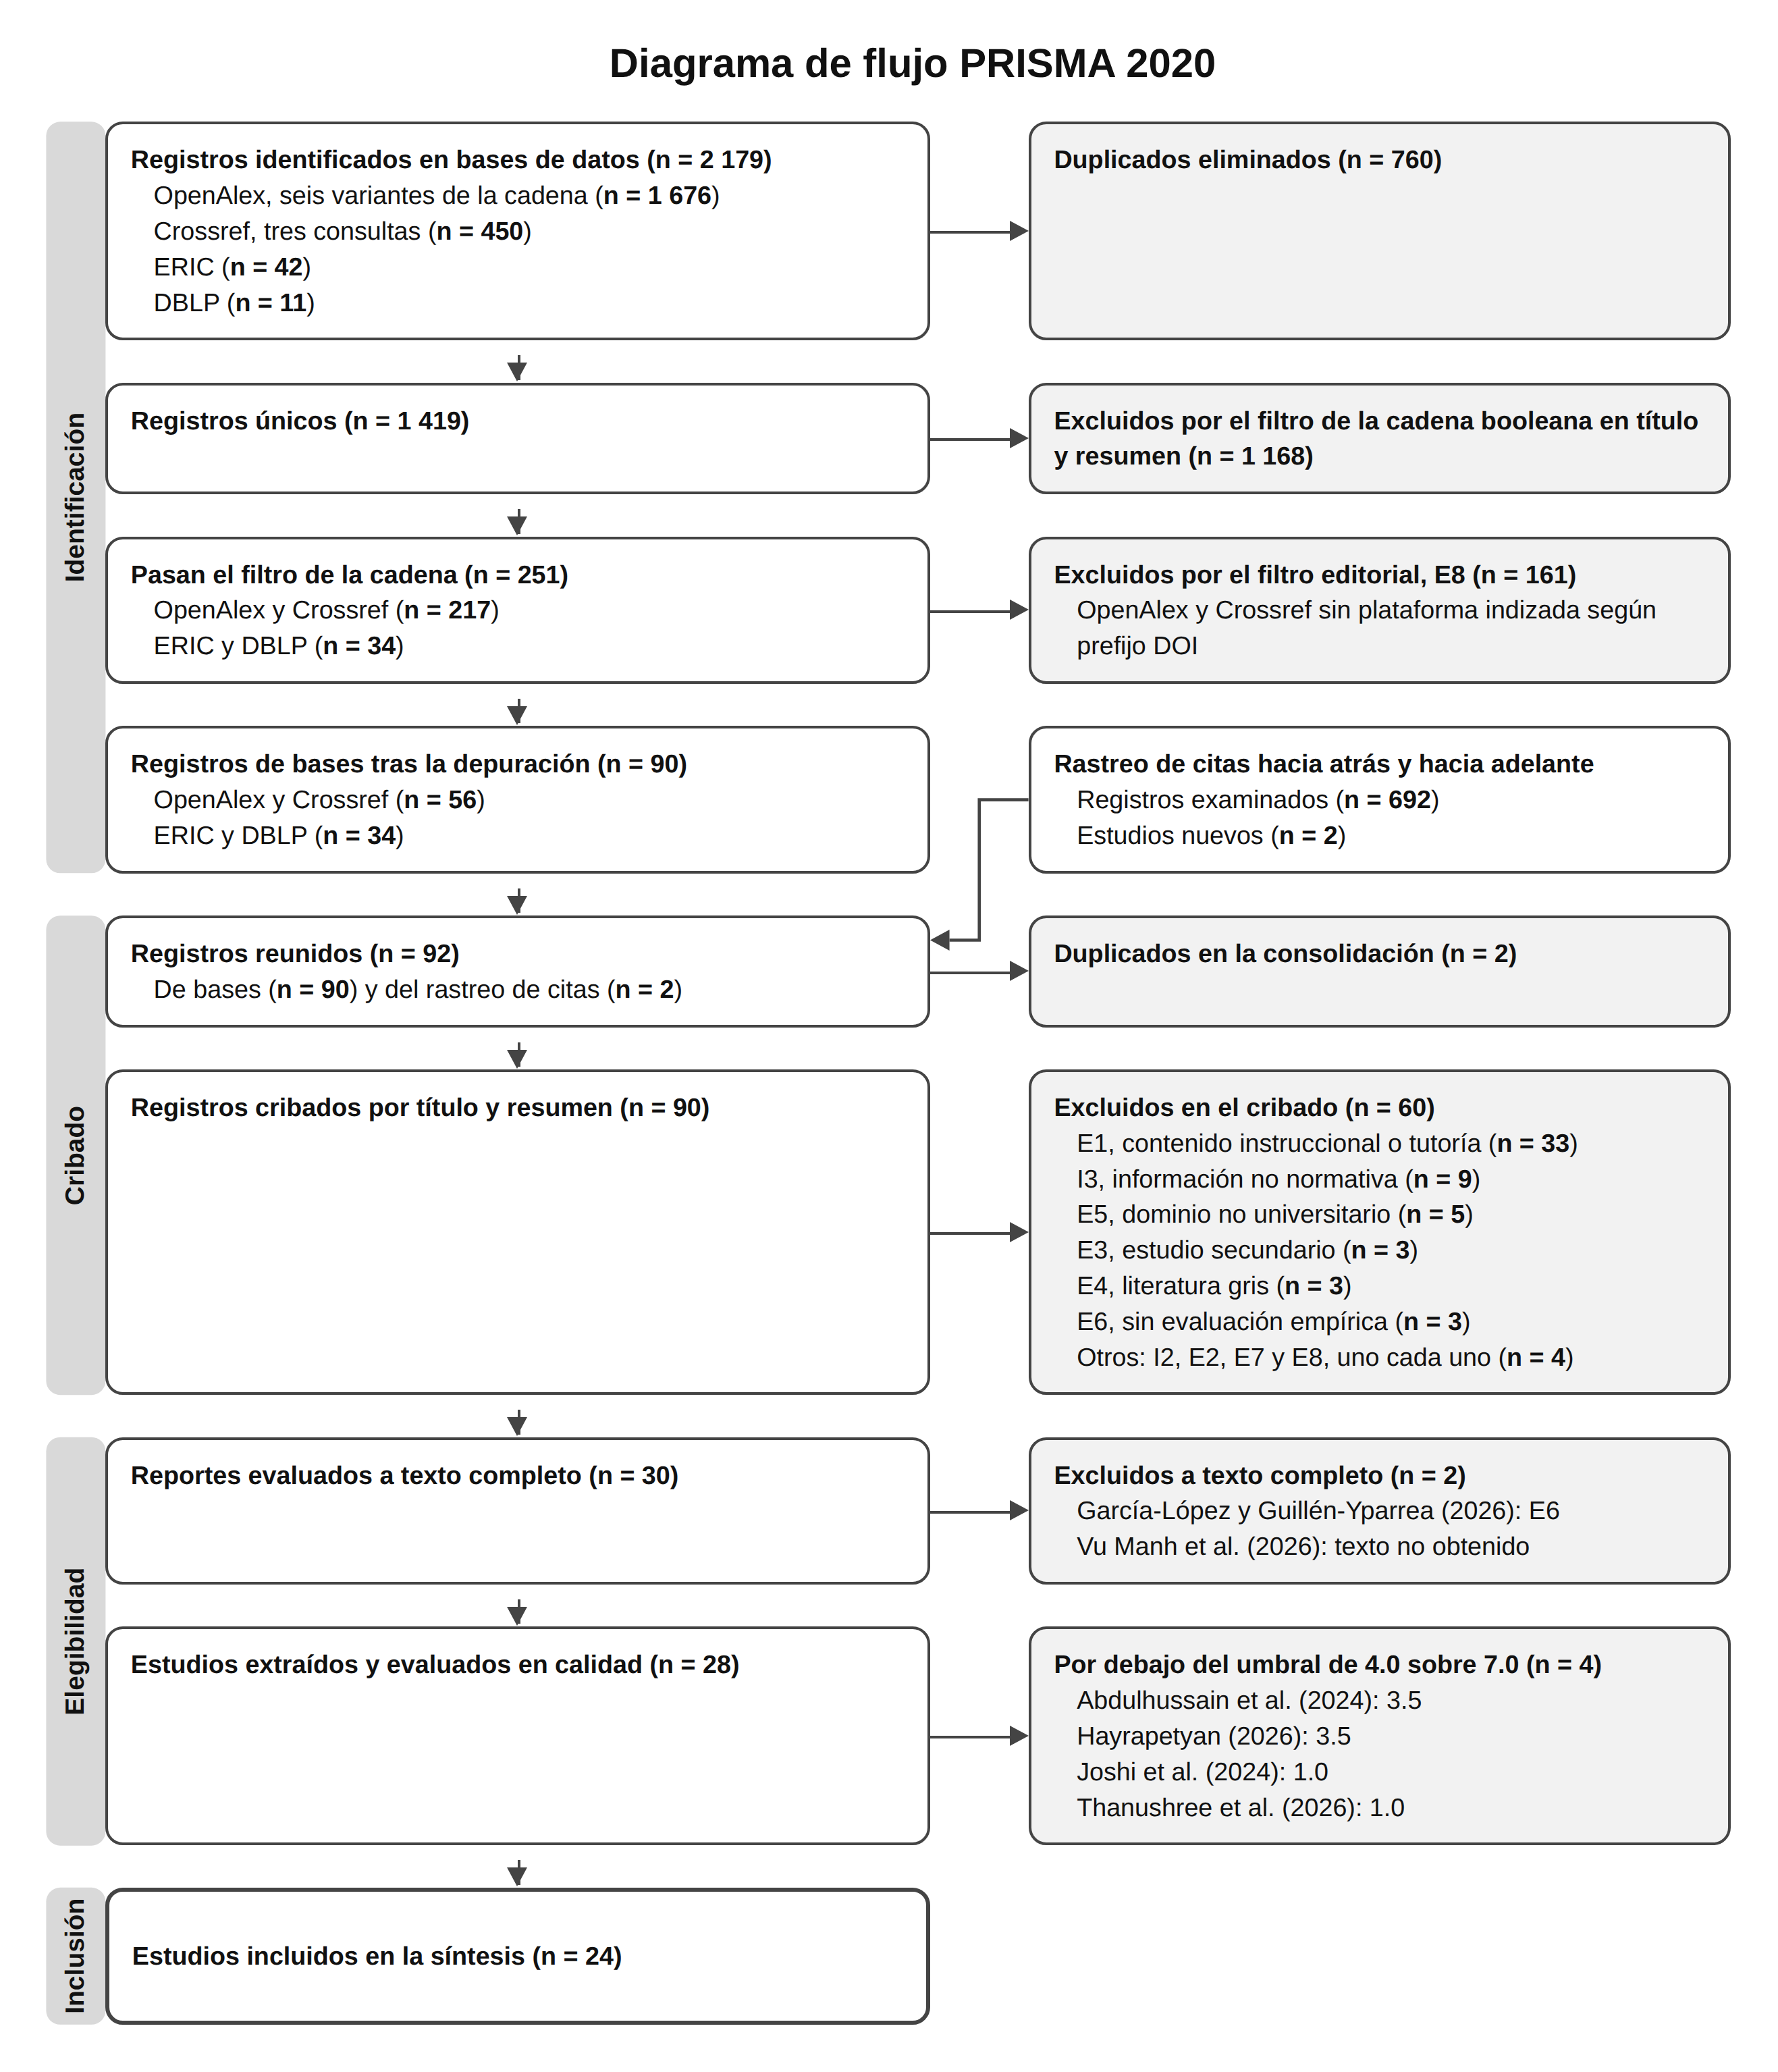
\includegraphics[width=0.9\textwidth]{diagrama_PRISMA.png}
\figurenote{Adaptado de \textcite{page2021}. Los motivos de exclusión se desglosan por criterio de elegibilidad. El filtro de la cadena booleana se aplicó de forma automatizada sobre título y resumen.}
\end{figure}

El cribado excluyó 60 estudios. E1 fue el motivo dominante, con 33 estudios que trataban contenido instruccional o tutoría en lugar de información institucional; siguieron I3 con 9 casos, E5 con 5, y E3, E4 y E6 con 3 cada uno.

De los 30 estudios evaluados a texto completo salieron dos.\footnote{Las referencias completas de los estudios excluidos se listan en el Apéndice A y B.} \textcite{garcialopez2026} habían superado el cribado por su resumen, pero el texto completo mostró un artefacto conceptual de ciencia del diseño sin evaluación empírica, cuyas puntuaciones de fiabilidad los propios autores declaran hipotéticas (criterio E6). El capítulo de \textcite{vumanh2026} no pudo obtenerse a texto completo; comparte autoría con \textcite{nguyenl2025}, que sí se incluyó. Se extrajeron 28 estudios y, al aplicar el umbral de calidad, cuatro quedaron por debajo de 4.0. La síntesis se construye sobre 24.

La cobertura de la búsqueda se estimó con un análisis de captura y recaptura contra el conjunto de una exploración previa con criterios amplios. De 37 estudios de ese conjunto que cumplen los criterios de plataforma y fecha de esta revisión, la búsqueda recuperó 23, lo que estima una recuperación de 62~\%. Los 14 no recuperados, casi todos ponencias de IEEE de 2025 y 2026, quedan documentados en el repositorio del proyecto para su cribado en la actualización de la revisión. El rastreo de citas, por su parte, aportó solo 2 estudios nuevos de 692 registros examinados.

\subsection{Características de los Estudios Incluidos}
\begin{table}[htbp]
\caption{Distribución de los 24 Estudios de la Síntesis}
\label{tab:2}
\small
\begin{tabular}{@{}>{\raggedright\arraybackslash}p{0.307\linewidth}>{\raggedright\arraybackslash}p{0.653\linewidth}@{}}
\toprule
Dimensión & Distribución \\ \midrule
Año & 2025: 14; 2024: 6; 2026: 4 \\
Tipo de publicación & Ponencia en congreso: 18; artículo de revista: 3; capítulo en acta indizada: 2; artículo en acta de revista: 1 \\
Editorial & IEEE: 16; ACM: 3; Springer: 2; MDPI: 2; Elsevier: 1 \\
País & Vietnam: 4; China: 3; Filipinas: 3; Indonesia: 2; Estados Unidos: 2; India: 2; Corea del Sur, Reino Unido, Rumania, Tailandia, Polonia, Bangladés, Rusia y Sri Lanka: 1 cada uno \\
Idioma del corpus & Inglés: 11 (uno bilingüe con coreano); vietnamita: 4; chino: 2; indonesio: 2; polaco, rumano, ruso y tailandés: 1 cada uno; no declarado: 1 \\
Despliegue del generador & Local: 12; servicio externo: 7; comparación de ambos: 1; no declarado: 4 \\
\bottomrule
\end{tabular}
\par\vspace{0.4ex}{\footnotesize\noindent\textit{Nota.} La editorial se determinó por el prefijo del identificador digital de objeto. El idioma bilingüe se cuenta en la categoría de inglés.\par}
\end{table}

Dieciocho de los 24 estudios son de 2025 o posteriores, y ninguno es anterior a 2024 aunque la ventana se abrió en 2022. El campo tiene menos de tres años, lo que explica a la vez su energía y su inmadurez metodológica.

Las ponencias de congreso dominan con 18 de 24. Solo tres estudios son artículos de revista con revisión completa, y los tres puntúan 6.0 o más en calidad, por encima de la mediana. La diferencia tiene más que ver con el espacio disponible que con el prestigio: un artículo de seis páginas no alcanza para describir un corpus, especificar una arquitectura, declarar un conjunto de prueba y construir una línea base. Varios vacíos de reporte documentados más adelante son, en parte, vacíos de extensión.

Ningún estudio de la síntesis trabaja con un corpus en español. Ninguno proviene de una institución latinoamericana con evaluación empírica, y el único trabajo mexicano recuperado fue el excluido por falta de evaluación. Dos de los estudios más cuidadosos de la muestra atienden precisamente lenguas con representación marginal en los modelos de partida: el trabajo rumano documenta que su modelo base contiene alrededor de 0.03~\% de datos en rumano, y el polaco construye su propio conjunto de evaluación porque los existentes no cubren documentos regulatorios en polaco. Este vacío constituye la razón de ser de la presente tesis.

Siete estudios se dirigen solo a aspirantes y seis solo a estudiantes inscritos. Solo dos tienen como usuario principal al personal de la institución, porque el esfuerzo se ha concentrado en la ventanilla de admisiones, que reúne el mayor volumen y la mayor estacionalidad.

\subsection{Calidad de los Estudios}
\begin{table}[htbp]
\caption{Puntuación de Calidad de los 24 Estudios de la Síntesis}
\label{tab:3}
\small
\begin{tabular}{@{}>{\raggedleft\arraybackslash}p{0.080\linewidth}>{\raggedleft\arraybackslash}p{0.080\linewidth}>{\raggedright\arraybackslash}p{0.780\linewidth}@{}}
\toprule
Puntuación & n & Estudios \\ \midrule
6.5 & 5 & \textcite{joldea2025}; \textcite{khasanova2025}; \textcite{quincoso2026}; \textcite{shaikh2025}; \textcite{wojtasik2025} \\
6.0 & 6 & \textcite{dayata2024}; \textcite{ekene2025}; \textcite{nguyenl2025}; \textcite{stepanov2026}; \textcite{tamascelli2025}; \textcite{van2025} \\
5.5 & 2 & \textcite{nguyenht2024}; \textcite{ramli2025} \\
5.0 & 4 & \textcite{jayakody2026}; \textcite{nguyenthidieu2024}; \textcite{xu2024}; \textcite{zhong2025} \\
4.5 & 3 & \textcite{artayasa2025}; \textcite{calfoforo2024}; \textcite{vurukonda2026} \\
4.0 & 4 & \textcite{comia2025}; \textcite{khan2025}; \textcite{rachmat2024}; \textcite{wu2025} \\
\bottomrule
\end{tabular}
\par\vspace{0.4ex}{\footnotesize\noindent\textit{Nota.} Puntuación máxima de 7.0. El umbral de inclusión en la síntesis fue 4.0.\par}
\end{table}

La media es 5.38 y la mediana 5.5. La distribución por criterio muestra un patrón muy marcado (Tabla 4).

\begin{table}[htbp]
\caption{Cumplimiento por Criterio de Calidad}
\label{tab:4}
\small
\begin{tabular}{@{}>{\raggedright\arraybackslash}p{0.580\linewidth}>{\raggedleft\arraybackslash}p{0.080\linewidth}>{\raggedleft\arraybackslash}p{0.080\linewidth}>{\raggedleft\arraybackslash}p{0.080\linewidth}>{\raggedleft\arraybackslash}p{0.080\linewidth}@{}}
\toprule
Criterio & Cumple & Parcial & No cumple & Media \\ \midrule
QA1. Objetivos claros & 22 & 2 & 0 & 0.96 \\
QA3. Arquitectura reproducible & 18 & 6 & 0 & 0.88 \\
QA5. Línea base o alternativa & 19 & 3 & 2 & 0.85 \\
QA4. Evaluación con métricas & 16 & 8 & 0 & 0.83 \\
QA6. Limitaciones discutidas & 16 & 8 & 0 & 0.83 \\
QA2. Corpus replicable & 14 & 10 & 0 & 0.79 \\
QA7. Datos o código disponibles & 4 & 3 & 17 & 0.23 \\
\bottomrule
\end{tabular}
\par\vspace{0.4ex}{\footnotesize\noindent\textit{Nota.} \emph{n} = 24. La media se calcula con 1 para cumple, 0.5 para parcial y 0 para no cumple.\par}
\end{table}

Seis criterios promedian 0.79 o más. El séptimo promedia 0.23. La disponibilidad de datos o código es el criterio que el campo incumple casi por completo, y la distancia respecto de los demás no se explica por falta de espacio: publicar un repositorio no consume páginas.

Los cuatro estudios que quedaron fuera por el umbral se listan en la Tabla 5, porque uno de ellos aporta un hallazgo que se recupera en la discusión.\footnote{Las referencias completas de los estudios excluidos se listan en el Apéndice A y B.}

\begin{table}[htbp]
\caption{Estudios por Debajo del Umbral de Calidad, Excluidos de la Síntesis}
\label{tab:5}
\small
\begin{tabular}{@{}>{\raggedright\arraybackslash}p{0.232\linewidth}>{\raggedleft\arraybackslash}p{0.080\linewidth}>{\raggedright\arraybackslash}p{0.628\linewidth}@{}}
\toprule
Estudio & Total & Motivo determinante \\ \midrule
\textcite{abdulhussain2024} & 3.5 & No evalúa las respuestas de su propio sistema; su tabla de desempeño reproduce valores de referencia públicos de los modelos. No declara tamaño de fragmento, valor de \emph{k} ni conjunto de prueba. \\
\textcite{hayrapetyan2026} & 3.5 & Ponencia corta que no describe la arquitectura que evalúa ni identifica sus modelos; no tiene línea base ni publica los registros analizados. \\
\textcite{joshi2024} & 1.0 & Enuncia seis métricas y no reporta el valor de ninguna. No identifica el modelo de representación ni el de lenguaje. \\
\textcite{thanushree2026} & 1.0 & No mide nada: su única tabla de resultados compara características frente a un proceso manual idealizado, y la mejora de más de 40~\% que anuncia el resumen no se deriva en el texto. \\
\bottomrule
\end{tabular}
\par\vspace{0.4ex}{\footnotesize\noindent\textit{Nota.} Puntuación máxima de 7.0. La justificación de cada criterio está disponible en el repositorio del proyecto.\par}
\end{table}

El último caso muestra por qué un umbral de calidad tiene que aplicarse y no quedarse en el protocolo. Con criterios amplios, un estudio que anuncia una mejora porcentual en su resumen sin medirla en el cuerpo habría entrado a la síntesis, y su cifra se habría propagado como evidencia.

\subsection{PI1. Arquitecturas y Preparación del Corpus}
\subsubsection{Segmentación del Documento}
Veinte de los 24 estudios declaran una estrategia de segmentación y cuatro no la reportan o prescinden de ella por diseño (Tabla 6). Predominan los fragmentos de tamaño fijo, de 500 a 1\,200 unidades léxicas o caracteres; les siguen el corte por unidad estructural del documento, la fragmentación semántica y, en un caso, la fragmentación manual por intención de consulta. Diecisiete estudios justifican su elección de forma sustantiva, dos con un argumento meramente operativo y cinco no la justifican.

{\def\baselinestretch{1}\small\selectfont
\begin{longtable}{@{}>{\raggedright\arraybackslash}p{0.310\linewidth}>{\raggedleft\arraybackslash}p{0.080\linewidth}>{\raggedright\arraybackslash}p{0.550\linewidth}@{}}
\caption{Estrategias de Segmentación del Documento en los Estudios de la Síntesis}\label{tab:6}\\
\toprule
Estrategia & n & Estudios \\
\midrule
\endfirsthead
\multicolumn{3}{@{}l}{\textit{Tabla 6 (continuación)}}\\
\toprule
Estrategia & n & Estudios \\
\midrule
\endhead
Tamaño fijo, de 500 a 1\,200 unidades, con o sin solapamiento & 8 & \textcite{artayasa2025}; \textcite{jayakody2026}; \textcite{nguyenthidieu2024}; \textcite{ramli2025}; \textcite{shaikh2025}; \textcite{stepanov2026}; \textcite{tamascelli2025}; \textcite{wu2025} \\
Tamaño fijo comparado como variable: 512 contra 4\,000 unidades & 1 & \textcite{wojtasik2025} \\
División recursiva contra semántica, comparadas como variable & 1 & \textcite{khasanova2025} \\
Unidad estructural: artículo, página o proposición & 3 & \textcite{dayata2024}, por artículo; \textcite{comia2025}, por página; \textcite{xu2024}, que reescribe cada oración como enunciado de un solo sujeto \\
Semántica, por similitud entre oraciones contiguas & 2 & \textcite{nguyenl2025}; \textcite{zhong2025} \\
Manual, organizada por intención de consulta & 1 & \textcite{nguyenht2024} \\
Declarada sin tamaño ni criterio de corte & 4 & \textcite{calfoforo2024}; \textcite{joldea2025}; \textcite{van2025}; \textcite{vurukonda2026} \\
No declarada o no aplicable & 4 & \textcite{ekene2025}; \textcite{khan2025}; \textcite{quincoso2026}; \textcite{rachmat2024} \\
\bottomrule
\end{longtable}}
\vspace{-1.2em}
{\footnotesize\noindent\textit{Nota.} \emph{n} = 24. \textcite{quincoso2026} representan la norma como esquema relacional y reglas lógicas, sin fragmentos de texto.\par}
\vspace{1em}

Solo dos estudios someten la segmentación a prueba experimental. \textcite{khasanova2025} la tratan como uno de los tres factores de un diseño con 23 configuraciones y dos conjuntos de evaluación, y la división semántica gana a la recursiva en las mejores configuraciones. \textcite{wojtasik2025} convierten el tamaño del fragmento en pregunta de investigación sobre 2\,350 documentos normativos y evalúan además dos formas de resumir el fragmento largo.

Sus resultados son el hallazgo más consecuente de esta revisión para la segmentación normativa. El fragmento de 512 unidades supera al de 4\,000 en recuperación y en generación, aunque la colección de fragmentos largos sea más pequeña y en principio más fácil de buscar. En recuperación, el mejor proceso alcanza una ganancia acumulada descontada normalizada en los primeros diez resultados (nDCG@10) de 82.03 con 512 unidades y de 76.39 con 4\,000; en generación, la puntuación total cae de 87.32 a 84.34, y la caída se explica por la calidad de la cita. Resumir el fragmento largo empeora todo. La puntuación baja a 66.27 con resumen abstractivo y a 70.42 con extractivo, porque la paráfrasis pierde información que la norma necesita conservar.

\textcite{nguyenl2025} reescriben cada fragmento con el contexto general del documento del que proviene, la idea más cercana a una representación jerárquica en toda la muestra. Con ella, un modelo abierto de 7 mil millones de parámetros alcanza 0.628 de exactitud contra 0.544 de GPT-4o, 0.502 de Claude 3.5 Sonnet y 0.440 de Gemini 1.5 Pro, evaluados estos en sus plataformas oficiales con acceso a internet.

\textcite{vurukonda2026} nombran y miden la colisión de contexto, que ocurre cuando dependencias de una misma universidad usan vocabulario idéntico para reglas distintas, como una calificación aprobatoria de 40~\% en una escuela y de 50~\% en otra. Separar el índice por dependencia redujo la alucinación de 14~\% a 3~\% y elevó la pertinencia contextual de 61~\% a 89~\%.

\subsubsection{Configuración de la Recuperación}
El modelo de representación más usado es \texttt{all-MiniLM-L6-v2}, presente en siete estudios, y cinco estudios no identifican el que emplean. El valor de \emph{k} se declara en 10 de los 24 estudios, con valores de 3 a 20, y subirlo de 5 a 10 eleva la exhaustividad de 0.80 a 0.95 a costa de bajar la precisión de 0.92 a 0.85 \parencite{nguyenthidieu2024}. Con fragmentos de 4\,000 unidades, BM25, una técnica de coincidencia léxica de los años setenta, superó a todos los recuperadores densos \parencite{wojtasik2025}. El documento normativo largo abunda en terminología específica, que es el régimen donde la coincidencia exacta aventaja a la similitud semántica.

El reordenamiento aparece en 6 de los 24 estudios, aunque donde se aísla su efecto es grande: el mismo recuperador pasa de 59.31 a 82.03 de nDCG@10 al añadirlo, sin cambio en la exhaustividad \parencite{wojtasik2025}. Los documentos correctos ya estaban en el conjunto recuperado; solo faltaba ordenarlos. Cuatro estudios combinan un canal léxico con uno denso, y dos añaden una representación en grafo con la que la pertinencia del contexto sube de 0.21 a entre 0.49 y 0.65 \parencite{zhong2025} y la exactitud con atribución en consultas de varios pasos de 0.55 a 0.91 \parencite{stepanov2026}. Los cuatro híbridos superan la mediana de calidad.

\subsubsection{Modelo Generador y Despliegue}
Llama es la familia generadora más frecuente, con doce estudios, seguida por los modelos de OpenAI con siete, y aparecen además Mistral, Gemini, Command-R-Plus, Qwen destilado, GLM-4, Bielik, OpenChat y LLaVA. Doce estudios despliegan el generador en infraestructura propia, sobre todo por soberanía de los datos y costo operativo. \textcite{jayakody2026} añaden un argumento práctico: los modelos con filtros de seguridad estrictos rechazan consultas burocráticas inocuas, como preguntar el procedimiento para apelar una suspensión. La evidencia sobre calidad es contraintuitiva y consistente, porque un modelo abierto bien optimizado alcanza 0.7377 de promedio frente al 0.7351 del modelo comercial de referencia \parencite{khasanova2025}. \textcite{nguyenl2025} llegan a una conclusión del mismo signo con un margen mayor. La lectura que hacen \textcite{jayakody2026} de su resultado como refutación de las leyes de escala va demasiado lejos, porque enfrentan un modelo anclado contra modelos sin anclaje y aíslan el efecto de la recuperación, no el del tamaño.

\subsection{PI2. Evaluación de la Fidelidad}
\subsubsection{Qué se Mide}
\begin{table}[htbp]
\caption{Familias de Métricas Empleadas en los Estudios de la Síntesis}
\label{tab:7}
\small
\begin{tabular}{@{}>{\raggedright\arraybackslash}p{0.473\linewidth}>{\raggedleft\arraybackslash}p{0.080\linewidth}>{\raggedright\arraybackslash}p{0.387\linewidth}@{}}
\toprule
Familia de métricas & n & Observación \\ \midrule
Clasificación: exactitud, precisión, exhaustividad, medida F & 12 & Familia dominante \\
Valoración humana: rúbrica, encuesta o juicio experto & 10 & Rara vez con protocolo declarado \\
Latencia y tiempo de respuesta & 7 & Siempre interna al sistema \\
Similitud de representaciones: coseno, BERTScore & 6 & Problemas de validez de constructo \\
Marco RAGAS & 5 & Específico de recuperación y generación \\
Léxicas: BLEU, ROUGE, METEOR & 5 & Miden solapamiento, no veracidad \\
Ordenamiento: MRR, nDCG, exhaustividad en los primeros \emph{k} & 5 & Presentes en estudios de calidad alta \\
Tasa de alucinación & 4 & La medida más directa del problema \\
Calidad de la cita & 2 & Casi inexistente \\
\bottomrule
\end{tabular}
\par\vspace{0.4ex}{\footnotesize\noindent\textit{Nota.} \emph{n} = 24. Un estudio puede emplear varias familias, por lo que las frecuencias no suman 24.\par}
\end{table}

La familia más usada es la de métricas de clasificación, importada de tareas de aprendizaje supervisado. Las métricas diseñadas para recuperación y generación aparecen en cinco estudios, y las que miden lo que más importa en el dominio normativo, la tasa de alucinación y la calidad de la cita, en cuatro y en dos.

Cuando la fidelidad se mide aparte de la pertinencia, resulta la puntuación más baja. \textcite{artayasa2025} reportan, sobre 50 consultas, una fidelidad de 0.7293 frente a una pertinencia de 0.8869 y una exhaustividad del contexto de 0.9078: el sistema encuentra el contexto y responde a la pregunta, pero se apega menos al documento. Calculada contra la respuesta de referencia en lugar del contexto, esa misma fidelidad baja a 0.6783.

En el estudio de \textcite{khasanova2025}, las puntuaciones altas de RAGAS coinciden con valores bajos de BLEU: su mejor configuración alcanza una pertinencia de 0.7606 con un BLEU de 0.0352 en el conjunto anotado a mano. Un estudio que reporte solo BLEU o ROUGE, y cinco lo hacen, no mide fidelidad en ningún sentido útil. \textcite{rachmat2024} reconocen que ROUGE mide solapamiento y no veracidad, aunque su ROUGE de 1.0 en 20 de 20 preguntas sugiere que el conjunto de prueba coincide con el de entrenamiento.

\subsubsection{Problemas de Validez de Constructo}
Dos estudios miden la fidelidad comparando la respuesta con el texto fuente. \textcite{comia2025} reporta una similitud media de 0.9219 entre la respuesta y el contenido oficial del manual, y \textcite{joldea2025} piden a un modelo de lenguaje una puntuación de 0 a 100 de similitud entre la respuesta y extractos del documento. El problema es el mismo en ambos casos. Medir la similitud entre la respuesta y el texto fuente premia la reproducción literal del documento y no la corrección de la respuesta a la pregunta: un sistema que devolviera íntegro el párrafo recuperado ante cualquier consulta obtendría una puntuación excelente sin haber respondido nada.

\textcite{comia2025} informa además un valor \emph{p} de 0.0000 como confirmación de significancia, sin indicar la hipótesis contrastada ni la prueba empleada, y no declara el tamaño de la muestra, que por la tabla de resultados parece de nueve preguntas.

\subsubsection{Buenas Prácticas Identificadas}
\textcite{stepanov2026} definen la exactitud factual con atribución, que exige que todas las afirmaciones de la respuesta sean consistentes con la fuente oficial y que la respuesta incluya una atribución válida; una respuesta cierta sin cita válida cuenta como incorrecta. Sobre 1\,012 consultas de tráfico real de una campaña de admisión, con dos anotadores independientes, su configuración anclada en grafo alcanza 0.91 frente a 0.55 de la recuperación híbrida convencional en consultas de varios pasos. Convertir la trazabilidad en condición de la corrección es la aportación conceptual más importante de la muestra.

\textcite{wojtasik2025} construyen una medida F de la cita sobre los fragmentos pertinentes y la combinan con una exactitud de inclusión y otra de exclusión de términos. Su conjunto de 100 preguntas se filtró desde casi 500 propuestas y se publica junto con el código de evaluación.

\textcite{shaikh2025} miden la alucinación con el mismo modelo como línea base: 31.7~\% de 160 consultas sin recuperación y 6.6~\% con ella. Dos anotadores independientes alcanzaron un kappa de Cohen de 0.84.

\textcite{ekene2025} presentan la única evaluación humana controlada de la muestra, con cinco evaluadores, protocolo ciego y un alfa de Cronbach de 0.82.

\textcite{tamascelli2025} repiten su evaluación en tres corridas, reportan la dispersión y declaran qué parte de sus pruebas no produce métricas.

\subsection{PI3. Evidencia Sobre la Reducción del Tiempo de Consulta}
Ocho de los 24 estudios reportan mediciones de tiempo. Ninguno compara el tiempo de consulta del sistema contra el mecanismo tradicional.

Lo que se mide, en los ocho casos, es tiempo interno al sistema. \textcite{ramli2025} reportan rangos de velocidad de generación de 7.56 a 68.67 segundos según el modelo y el entorno de ejecución. \textcite{stepanov2026} reportan latencia media, mediana y de percentil 95 por nivel de su arquitectura, con 0.47, 0.32 y 0.85 segundos en el nivel determinista y 4.80, 3.60 y 9.20 en el anclado en grafo. \textcite{khasanova2025} desglosan la latencia por etapa y muestran que optimizar la calidad la encarece: la recuperación pasa de 0.0053 a 6.1295 segundos y la generación de 1.221 a 9.1957. \textcite{quincoso2026} reportan 32.99 segundos por consulta contra 20.13 del modelo sin anclaje, y \textcite{shaikh2025} una media de 13.57 segundos con desviación de 10.87. \textcite{rachmat2024} reportan de 5 a 6 minutos por consulta, \textcite{van2025} unos 25 minutos por cada 100 consultas, y \textcite{calfoforo2024} reportan tiempo de entrenamiento y no de consulta.

Todas esas cifras comparan una configuración contra otra o son valores absolutos sin referente. El único trabajo recuperado que afirmó una mejora frente al proceso manual, de «más de 40~\% en eficiencia», quedó fuera por el umbral de calidad. La cifra no aparece sustentada en ninguna parte del texto.

Existe evidencia indirecta de valor operativo. \textcite{stepanov2026} reportan que el primer nivel de su arquitectura resuelve 68.7~\% de las peticiones de tráfico real con latencia inferior al segundo, un indicador legítimo de descarga de demanda aunque no mida el tiempo del usuario. \textcite{shaikh2025} reportan una satisfacción de 4.26 sobre 5 en 52 participantes. \textcite{van2025} encuestaron a 500 aspirantes: 86~\% declaró que el sistema aclaró sus dudas y la confianza para decidir promedió 4.12, con desviación de 0.74, aunque 12~\% valoró la experiencia de forma negativa, un dato que casi ningún otro estudio reporta.

La pregunta que justifica buena parte de estos sistemas, si reducen el tiempo de acceso a la información institucional, permanece sin respuesta empírica.

El diseño mínimo para cerrar este vacío no requiere sofisticación técnica. Basta un estudio con dos brazos, consulta asistida y consulta tradicional, sobre el mismo conjunto de preguntas y con medición del tiempo hasta obtener una respuesta correcta y verificable. Este diseño constituye el componente evaluativo central de la fase empírica de la tesis.

\subsection{PI4. Prácticas de Reporte y Vacíos Metodológicos}
\begin{table}[htbp]
\caption{Prácticas de Reporte en los 24 Estudios de la Síntesis}
\label{tab:8}
\small
\begin{tabular}{@{}>{\raggedright\arraybackslash}p{0.680\linewidth}>{\raggedleft\arraybackslash}p{0.080\linewidth}>{\raggedleft\arraybackslash}p{0.080\linewidth}>{\raggedleft\arraybackslash}p{0.080\linewidth}@{}}
\toprule
Práctica & Sí & Parcial & No \\ \midrule
La respuesta cita su fuente & 9 & 6 & 9 \\
La cita permite al usuario verificar & 8 & 1 & 15 \\
Hay línea base o configuración alternativa & 19 & 3 & 2 \\
Se declara el tamaño del conjunto de prueba & 17 & 0 & 7 \\
Se declara el volumen del corpus & 13 & 0 & 11 \\
Se declara el valor de \emph{k} & 10 & 0 & 14 \\
Se publican datos, código o conjunto de evaluación & 4 & 3 & 17 \\
\bottomrule
\end{tabular}
\par\vspace{0.4ex}{\footnotesize\noindent\textit{Nota.} \emph{n} = 24. En el valor de \emph{k} se cuenta como declarado solo el valor explícito; un estudio que no usa fragmentos de texto se cuenta en la columna No.\par}
\end{table}

La trazabilidad está lejos de ser la norma: la respuesta cita su fuente en 9 estudios y permite verificarla en 8, aunque citar es justo la ventaja que distingue a estos sistemas de un modelo sin anclaje. En el dominio normativo, una respuesta sobre un plazo de apelación sin referencia al artículo que lo fija no sirve para tomar una decisión.

\textcite{stepanov2026} son los únicos que gestionan la vigencia de la norma por diseño, con intervalos de validez por fragmento y una regla de precedencia entre el dato estructurado y el derivado de documentos. Los otros 23 estudios tratan el corpus como si fuera estático, aunque un reglamento se reforme y una convocatoria expire.

Diecisiete de 24 estudios no publican datos, código ni conjunto de evaluación, y solo cuatro lo hacen \parencite{dayata2024,joldea2025,quincoso2026,wojtasik2025}. Con 71~\% de no disponibilidad, los valores numéricos de esta revisión se leen como declaraciones de los autores.

Siete estudios no declaran el tamaño de su conjunto de prueba. La lectura del texto completo detectó además dos inconsistencias internas, de 46 contra 56 preguntas en un caso y de 680 contra 420 consultas en otro.

Los conjuntos declarados van de 3 a 5\,000 preguntas, con mediana de 100, y solo seis se construyen con preguntas reales de usuarios. \textcite{khasanova2025} muestran por qué importa la procedencia: su conjunto generado por modelo puntúa más alto que el anotado a mano porque sus preguntas están atadas al texto fuente.

\section{Discusión}
\subsection{Lo que la Literatura ha Establecido}
Tres afirmaciones cuentan con evidencia convergente de varios estudios con diseño comparativo.

El anclaje documental reduce la invención de datos. La tasa de alucinación baja de 31.7~\% a 6.6~\% con el mismo modelo \parencite{shaikh2025}, de 14~\% a 3~\% al particionar el índice \parencite{vurukonda2026} y de 0.15 a 0.00 en un conjunto reducido \parencite{ekene2025}. Un modelo sin anclaje propone asignaturas inelegibles o inexistentes con exactitud cercana a cero, mientras el mismo modelo con validación simbólica alcanza entre 0.81 y 0.83 \parencite{quincoso2026}.

La precisión de la recuperación pesa más que el tamaño del modelo generador. Tres estudios con diseños distintos llegan a esa conclusión, y \textcite{jayakody2026} la refuerzan con un análisis de error: de las fallas restantes de su sistema, 36~\% son de recuperación y 50~\% de síntesis con el contexto correcto ya entregado. Para una institución con presupuesto limitado, el gasto rinde más en la preparación del corpus y en la recuperación que en el modelo.

La estructura del documento fuente domina el resultado. \textcite{ramli2025} lo formulan a partir de su experiencia de implementación: las páginas largas y mal segmentadas y las tablas densas degradan la recuperación, y los documentos limpios con una fragmentación sensata mejoran el anclaje de inmediato. \textcite{wojtasik2025} lo confirman con el tamaño del fragmento, \textcite{zhong2025} con la representación estructurada y \textcite{vurukonda2026} con la partición del índice.

\subsection{Vacíos y Agenda de Trabajo}
\textbf{Vacío 1. Tiempo de consulta.} Es el vacío más llamativo, porque la reducción del tiempo de acceso es la justificación más repetida en las introducciones de estos estudios. Ocho miden tiempo y ninguno lo compara contra la ventanilla. Este vacío constituye el objetivo central de la fase empírica de esta tesis: un diseño de dos brazos que compare la consulta asistida contra la ventanilla tradicional sobre el mismo conjunto de preguntas normativas de la Universidad Autónoma de Guerrero.

\textbf{Vacío 2. Segmentación del documento normativo.} Veinte estudios declaran una estrategia y dos la prueban. La evidencia de esos dos apunta a fragmentos finos, sin resumen intermedio y con el contexto del documento incorporado, pero proviene de un corpus polaco y de uno coreano. Nadie ha probado si la estructura jerárquica del documento normativo, con título, capítulo, artículo y fracción, sirve mejor como criterio de corte que un tamaño fijo. La tesis abordará este vacío directamente: se construirá un corpus normativo en español de la Universidad Autónoma de Guerrero y se someterá la estrategia de segmentación a prueba experimental, explotando esa estructura jerárquica como criterio de corte.

\textbf{Vacío 3. Trazabilidad y vigencia.} Ocho de 24 estudios permiten verificar la respuesta en la fuente, y uno solo gestiona la vigencia de la norma. En un dominio donde la norma cambia por partes, una respuesta desactualizada hace tanto daño como una incorrecta. El sistema que se desarrolla en esta tesis incorpora trazabilidad verificable y gestión de vigencia como requisitos de diseño, no como características opcionales.

\textbf{Vacío 4. Instrumentos de fidelidad.} Doce estudios usan métricas de clasificación, cinco usan métricas de solapamiento léxico que sus propios usuarios reconocen inadecuadas y dos miden la similitud con el texto fuente, lo que premia la copia. Solo dos construyen una métrica de calidad de la cita. Se adoptará y adaptará el instrumento de exactitud factual con atribución propuesto por \textcite{stepanov2026}, que trata la cita como condición de la corrección.

\textbf{Vacío 5. Reproducibilidad.} El criterio de disponibilidad de datos promedia 0.23 sobre 1.00, frente a 0.79 o más en los otros seis. La asimetría apunta a una práctica establecida del campo y no a un problema de espacio ni de competencia metodológica. El protocolo, las cadenas de búsqueda, la matriz de extracción y el código del sistema se publican en repositorio abierto, en contraste con el 71~\% de la literatura revisada que no publica nada.

\textbf{Vacío 6. Español y América Latina.} Ningún estudio de la síntesis trabaja con corpus en español ni proviene de una institución latinoamericana con evaluación empírica. Los dos estudios más rigurosos sobre lenguas marginales en los modelos de partida documentan que esa marginalidad afecta el desempeño, así que no hay base para suponer que los resultados sobre corpus en inglés se transfieran sin pérdida al español. Este es el vacío que la tesis llena por definición: el primer estudio empírico de un sistema RAG sobre un corpus normativo universitario en español, en una institución pública latinoamericana.

\subsection{Implicaciones para la Implementación Institucional}
La lectura conjunta de la evidencia deja cinco decisiones de diseño con respaldo empírico.

Conviene fragmentar fino y no resumir. La evidencia favorece fragmentos del orden de 512 unidades léxicas sobre fragmentos de miles, y muestra que resumir el fragmento largo degrada la recuperación y la generación.

El fragmento debe cargar el contexto del documento del que proviene. Así se recupera mejor y permite citar con más precisión que un fragmento suelto.

El reordenador es el componente con mejor relación entre costo y ganancia de toda la arquitectura. En el único estudio que lo aísla aporta 22.72 puntos de nDCG@10, porque los documentos correctos suelen estar ya en el conjunto recuperado y solo mal ordenados.

Separar el índice por dependencia o por cuerpo normativo mitiga la colisión de contexto entre reglamentos que usan el mismo vocabulario para reglas distintas. El fenómeno está medido.

La cita forma parte de la respuesta y debe medirse como tal. Una respuesta cierta sin atribución válida no sirve para una decisión normativa, y ya existe un instrumento publicado que la cuenta como incorrecta.

Estas cinco decisiones constituyen los requisitos de diseño del sistema que se desarrolla en la fase empírica de esta tesis.

\subsection{Advertencia Sobre Fidelidad y Utilidad}
Dos estudios documentan de forma independiente que exigir fidelidad tiene un costo en utilidad. \textcite{tamascelli2025} relatan que las primeras versiones de su sistema fabricaban información, y que la ingeniería de instrucciones que corrigió el problema, restringir el modelo al contenido del manual, lo volvió tan cauteloso que respondía «no sé» con frecuencia ante preguntas sin respuesta directa en el documento. \textcite{wojtasik2025} encuentran el mismo fenómeno por otra vía: con una instrucción simple, exigir la cita redujo la corrección de la respuesta en todos los modelos probados sobre fragmentos de 512 unidades, y solo una instrucción más elaborada, que pide analizar los documentos antes de responder, revirtió la pérdida.

Fidelidad y utilidad no están alineadas por defecto. Un sistema que responde «no sé» a la mitad de las preguntas puede obtener una fidelidad excelente, de modo que cualquier reporte de fidelidad debe acompañarse de la tasa de abstención o de respuesta útil.

\section{Limitaciones}
La revisión se ejecutó con un solo revisor; la justificación de cada puntuación se publica para auditoría externa. La verificación de indización se realizó por prefijo de identificador digital, y la comprobación directa en Scopus y Web of Science queda pendiente. Un análisis de captura y recaptura estimó una recuperación de 62~\%, y los 14 estudios no recuperados se incorporarán en la actualización de la revisión. Un capítulo elegible \parencite{vumanh2026} no se obtuvo a texto completo. La heterogeneidad de métricas impide el metaanálisis, por lo que la síntesis es narrativa y tabular. La exclusión de literatura gris introduce sesgo de publicación a cambio de garantizar revisión por pares en todo el conjunto. Dieciocho de los 24 estudios son de 2025 o posteriores, y una revisión del mismo tema en dos años encontrará un panorama distinto.

\section{Conclusiones}
Esta revisión examinó la evidencia empírica sobre sistemas conversacionales anclados en recuperación aplicados al acceso a información normativa, administrativa y procedimental en universidades. De 2\,179 registros recuperados, 24 estudios con calidad metodológica suficiente conformaron la síntesis.

El campo ya estableció que el anclaje documental reduce de forma sustancial la invención de datos, que la precisión de la recuperación pesa más que el tamaño del modelo y que la estructura del documento fuente domina el resultado. Esas afirmaciones cuentan con evidencia convergente de diseños comparativos independientes y bastan para justificar la adopción de la técnica en el dominio normativo.

Lo que falta establecer es más interesante para quien vaya a implementar. No hay evidencia empírica de que estos sistemas reduzcan el tiempo de acceso a la información institucional, porque ocho de 24 estudios miden tiempo y ninguno lo compara contra la consulta tradicional. La segmentación del documento normativo casi no se ha investigado como variable, y la evidencia disponible proviene de corpus en lenguas distintas del español. La trazabilidad verificable es minoritaria y la vigencia normativa la gestiona por diseño un solo estudio. Diecisiete de 24 estudios no publican datos, código ni conjunto de evaluación, y ninguno trabaja con un corpus en español o proviene de América Latina.

Las dos líneas con mayor retorno metodológico pendiente, la segmentación del documento normativo en español y la medición del tiempo de acceso con diseño de dos brazos, constituyen los objetivos centrales de la fase empírica de esta tesis.

\section*{Referencias}
\printbibliography[heading=none,notkeyword=excluidocalidad,notkeyword=excluidotexto]

\section*{Apéndice A}
{\centering\textbf{Referencias de Estudios Excluidos por Calidad}\par}
\printbibliography[heading=none,keyword=excluidocalidad]

\section*{Apéndice B}
{\centering\textbf{Referencias de Estudios Excluidos en Texto Completo}\par}
\printbibliography[heading=none,keyword=excluidotexto]

\end{document}
